% ---------------------------------------------------------------------------
\section{Results}
\label{sec:results}
% ---------------------------------------------------------------------------

% ---------------------------------------------------------------------------
\subsection{Design Space and Objective Space Structure}
\label{sec:ground-truth-objectives}
% ---------------------------------------------------------------------------

\begin{figure}[htbp]
    \centering
    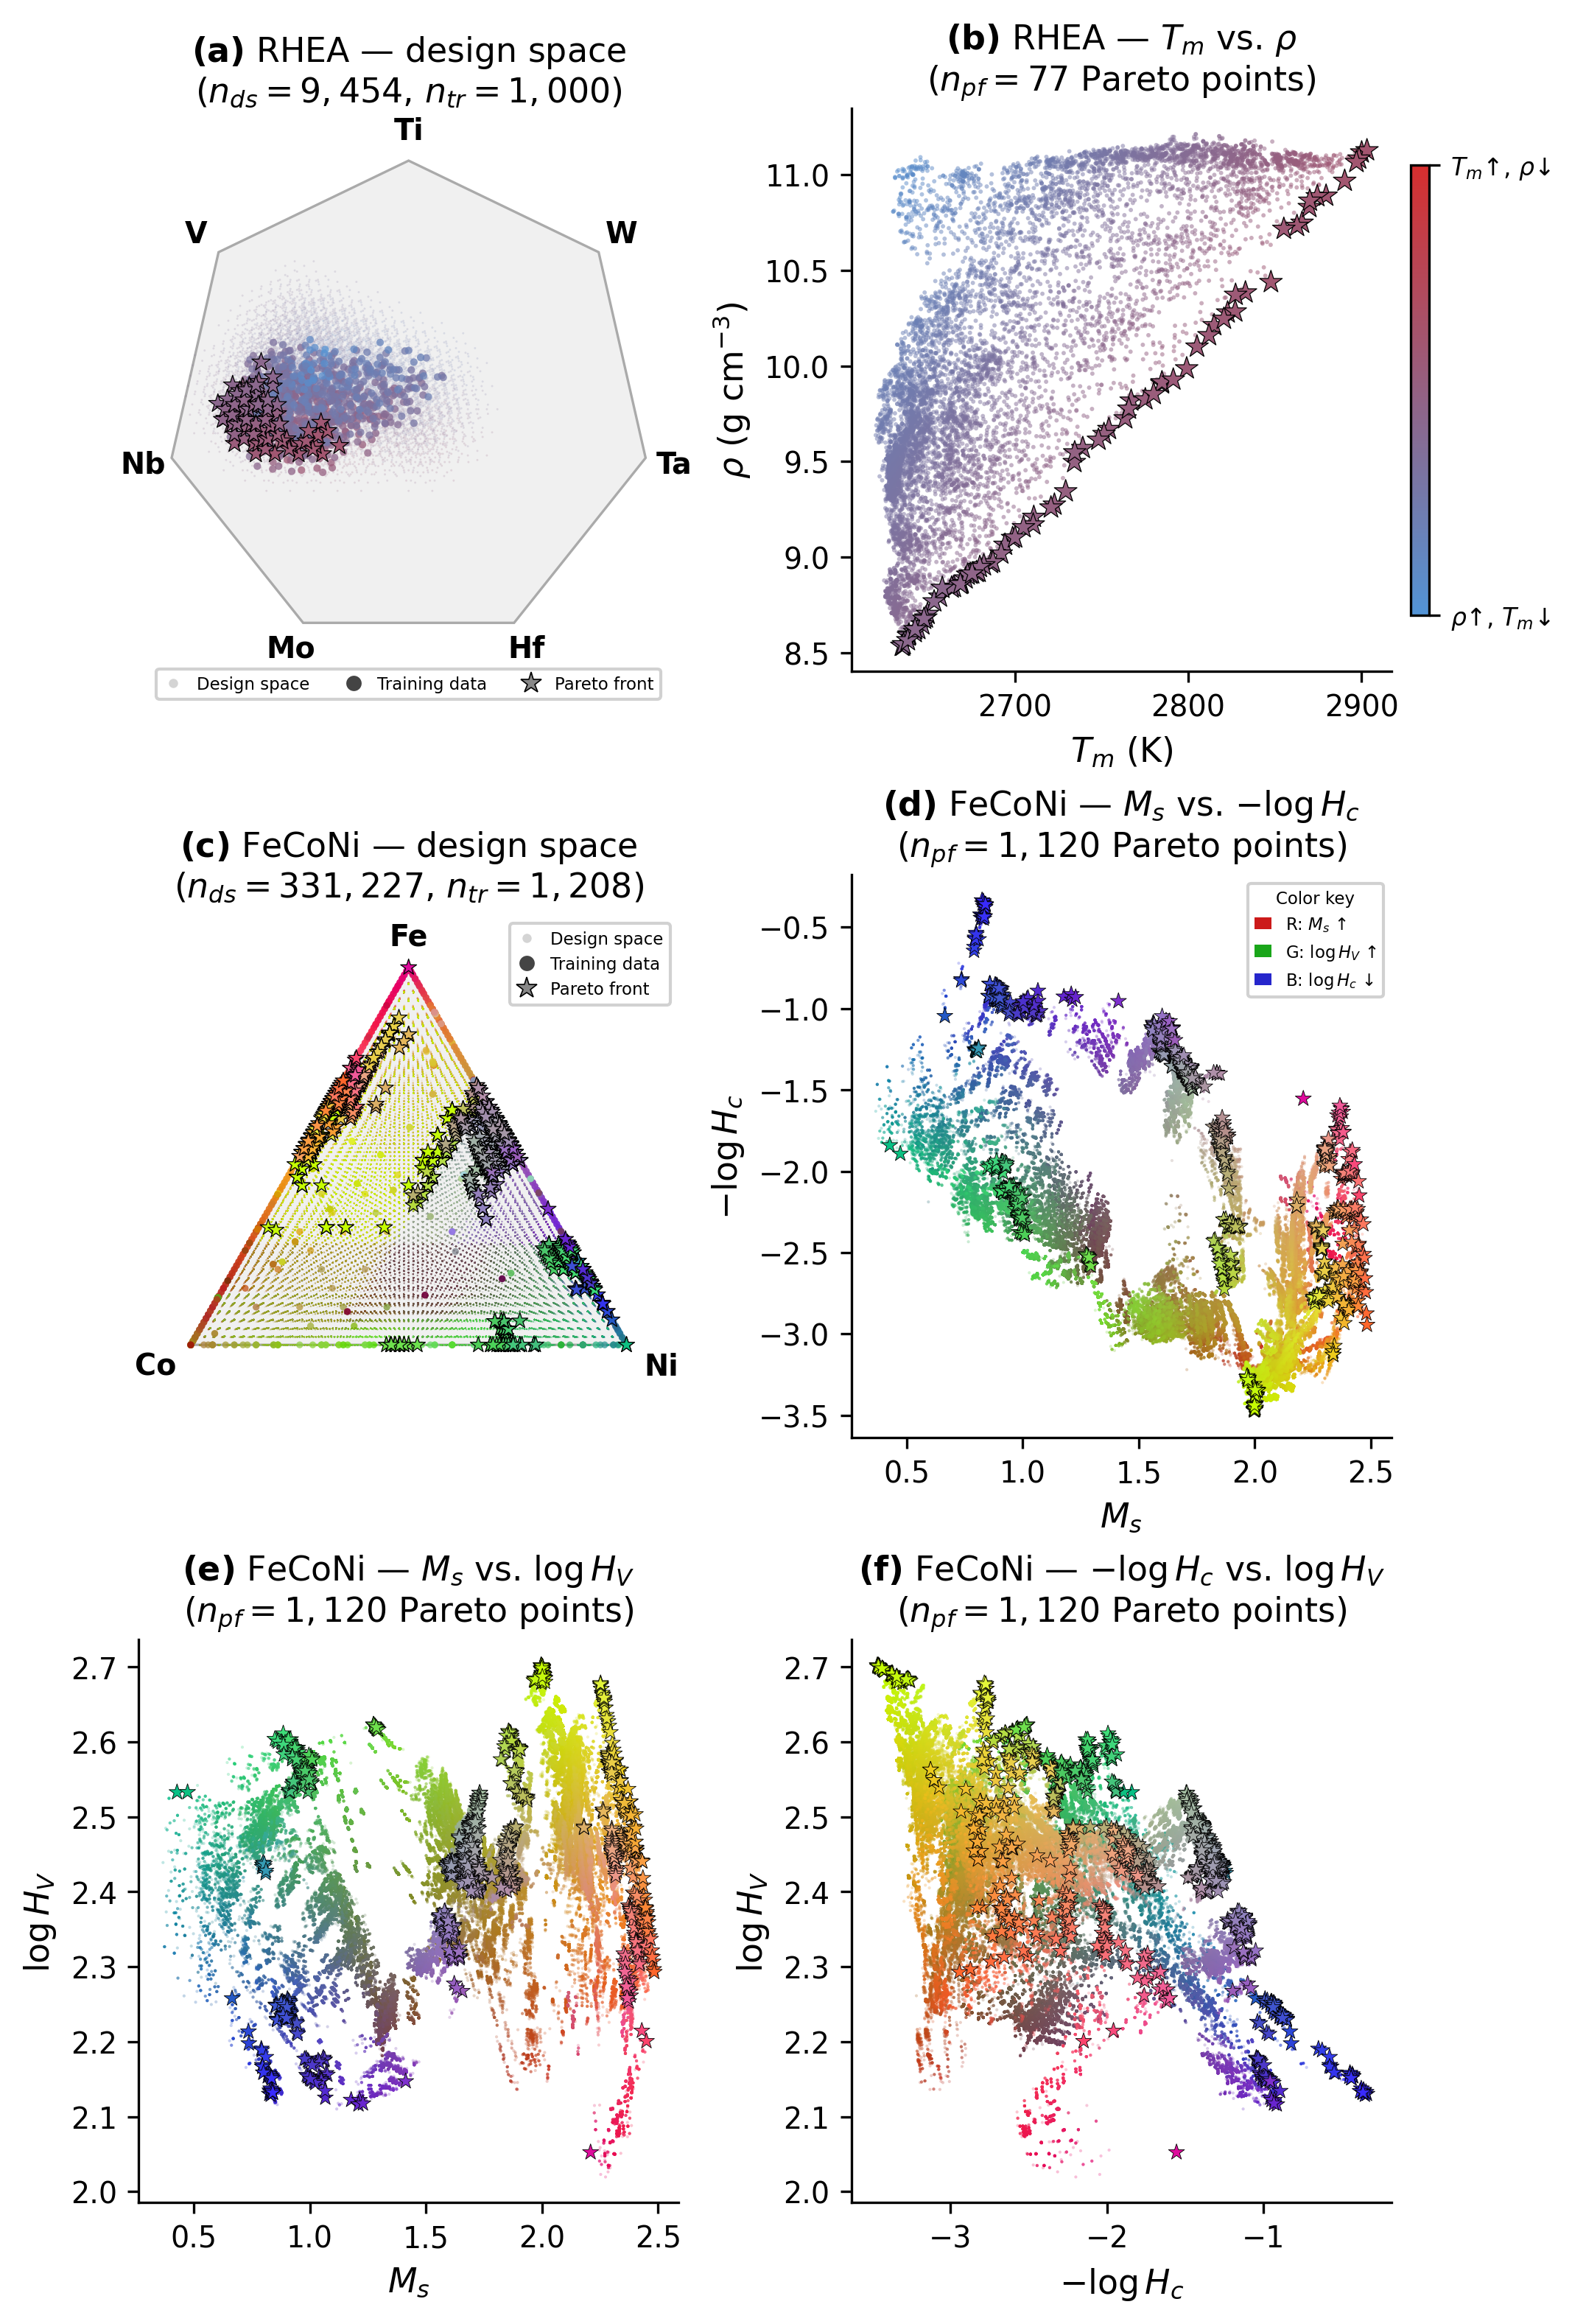
\includegraphics[width=0.9\linewidth]{figures/fig3_design_space.png}
    \caption{Ground-truth design and objective spaces for both systems.
             \textbf{(a)} RHEA system: training data and Pareto-optimal compositions shown in the septenary composition simplex.
             \textbf{(b)} RHEA objective space: density vs.\ melting temperature for all compositions, with Pareto-optimal points highlighted.
             \textbf{(c)} Fe-Co-Ni magnet system: training data and Pareto-optimal compositions projected onto the Fe--Co--Ni ternary, with Pareto-optimal compositions highlighted.
             \textbf{(d--f)} Fe-Co-Ni magnet objective space: pairwise projections of the three objectives, showing the multi-clustered structure of the Pareto front.}
    \label{fig:design-objectives}
\end{figure}

The RHEA and Fe-Co-Ni magnet problem design spaces were evaluated using the developed ground truth models to explore the actual Pareto fronts the strategies tried to discover. Fig.~\ref{fig:design-objectives} shows the composition and objective spaces for both systems.

The RHEA problem is focused on a relatively small contiguous cluster within the septenary simplex. Training data and Pareto-optimal compositions form a tight family of neighboring points in composition space, visible in panel (a). This spatial concentration carries over directly into the objective space in panel (b), where the density--melting temperature Pareto front spans a smooth and nearly linear tradeoff, with all optimal compositions grouped in a compact cluster. The optimization problem here is essentially one of locating and refining within a focused, well-connected region of the design space, a characteristic that distinguishes it from the Fe-Co-Ni magnet problem and will bear on interpreting the performance differences between them.

In contrast, the Fe-Co-Ni magnet problem looks quite different. Training data, shown in panel (c), is extensive along the binary edges of the ternary representation but becomes sparse in the interior. Despite this uneven coverage, the Pareto-optimal points clustered along specific binary edges and within isolated regions of the ternary interior, with clear discontinuities between groups. The three objective-space projections in panels (d)--(f) reinforce this picture, with every projection showing multiple distinct clusters of Pareto-optimal points rather than a continuous front. The optimization problem here involves finding and navigating a fragmented, multi-modal landscape substantially larger than the RHEA design space, representative of materials systems where the Pareto front is discontinuous and difficult to discover in full.

These two systems were chosen to represent qualitatively different optimization scenarios, with one presenting a compact and smooth landscape and the other a large and multi-clustered one, to stress-test fixed and adaptive resource-allocation strategies under different regimes. The experiments that follow probe whether strategy choice matters differently depending on which regime the campaign is operating in.
Using these ground truth models, we evaluate Adaptive-$\beta$, Rule-Swap, qEHVI, and Fixed Mixed across all eight experimental configurations described in Section~\ref{sec:experimental-design}, for both alloy systems.

% ---------------------------------------------------------------------------
\subsection{Baseline Optimization Performance}
\label{sec:results-baseline}
% ---------------------------------------------------------------------------

\begin{figure}[htbp]
    \centering
    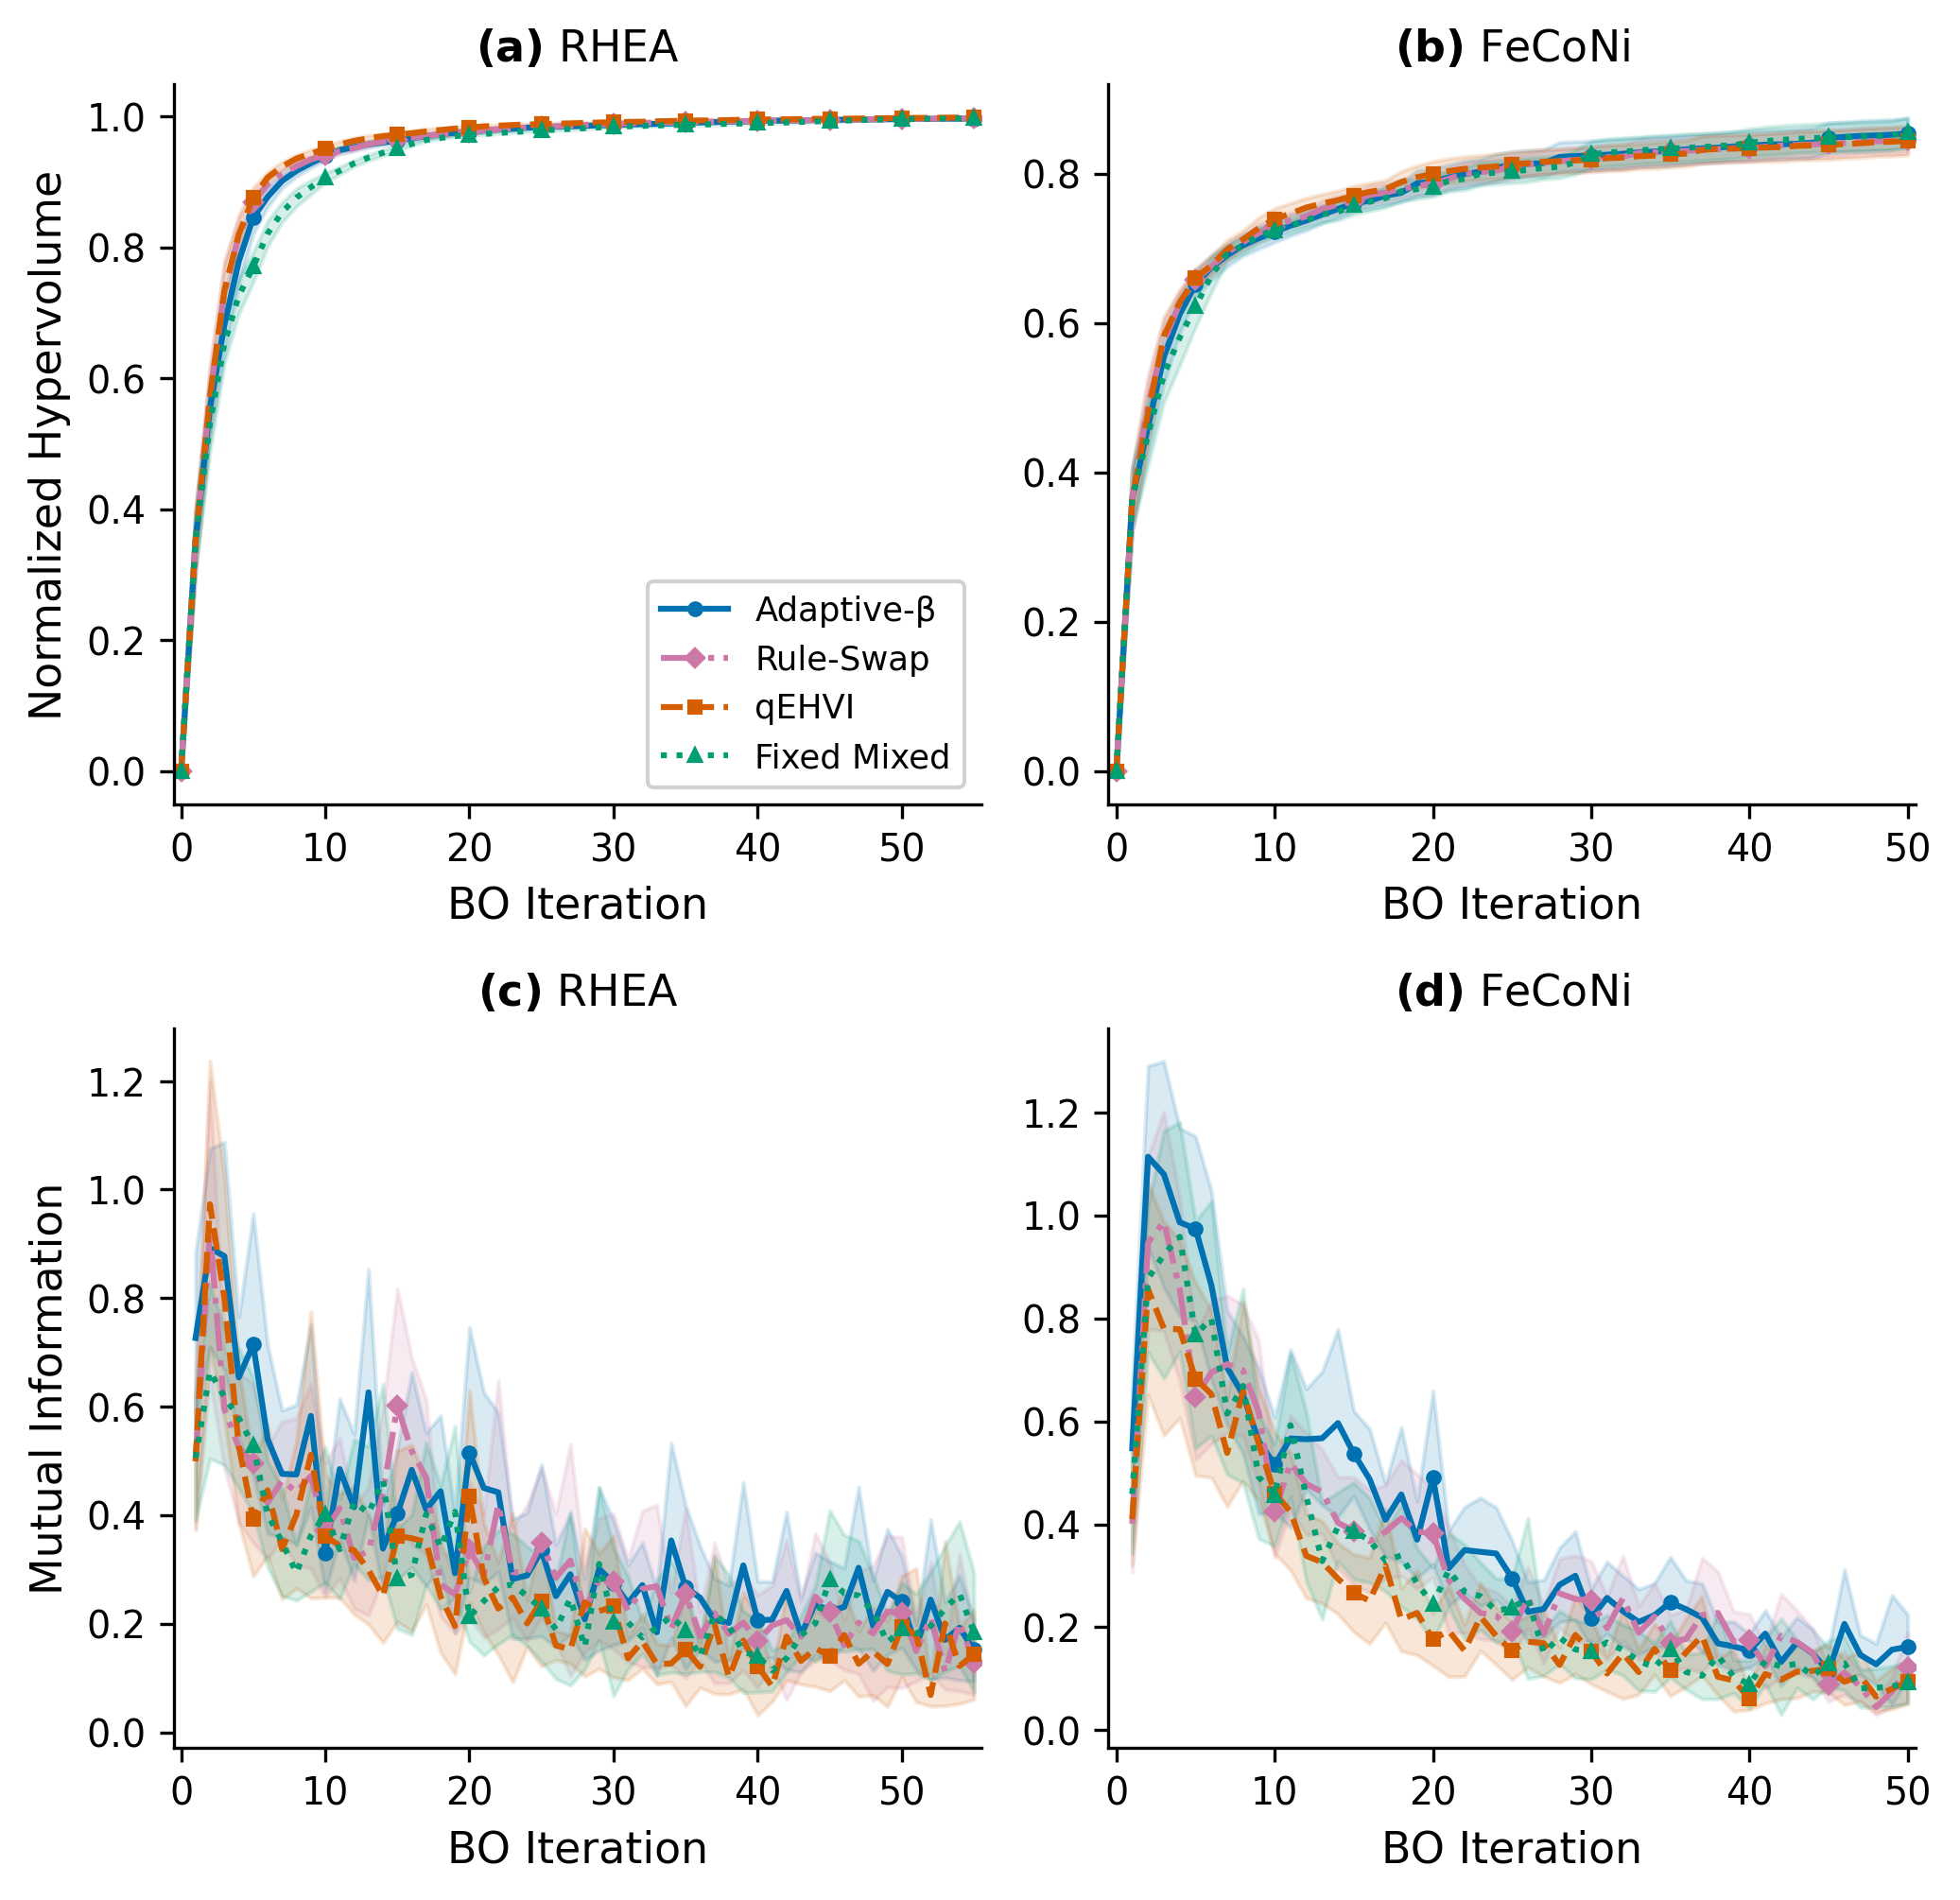
\includegraphics[width=\textwidth]{figures/fig4_baseline_combined.png}
    \caption{Baseline campaign results for both alloy systems with no resource events ($n = 25$ seeds per strategy).
             \textbf{a--b:} Hypervolume convergence; lines show per-strategy means and shaded bands indicate 95\% confidence intervals.
             \textbf{c--d:} Per-iteration mutual information across seeds; shaded bands are 95\% confidence intervals.
             Left column: RHEA system ($q = 5$, 55 iterations).
             Right column: Fe-Co-Ni magnet system ($q = 5$, 50 iterations).
             Strategies: Adaptive-$\beta$ (blue), Rule-Swap (purple), qEHVI (orange), Fixed Mixed (green).}
    \label{fig:baseline}
\end{figure}

\begin{figure}[htbp]
    \centering
    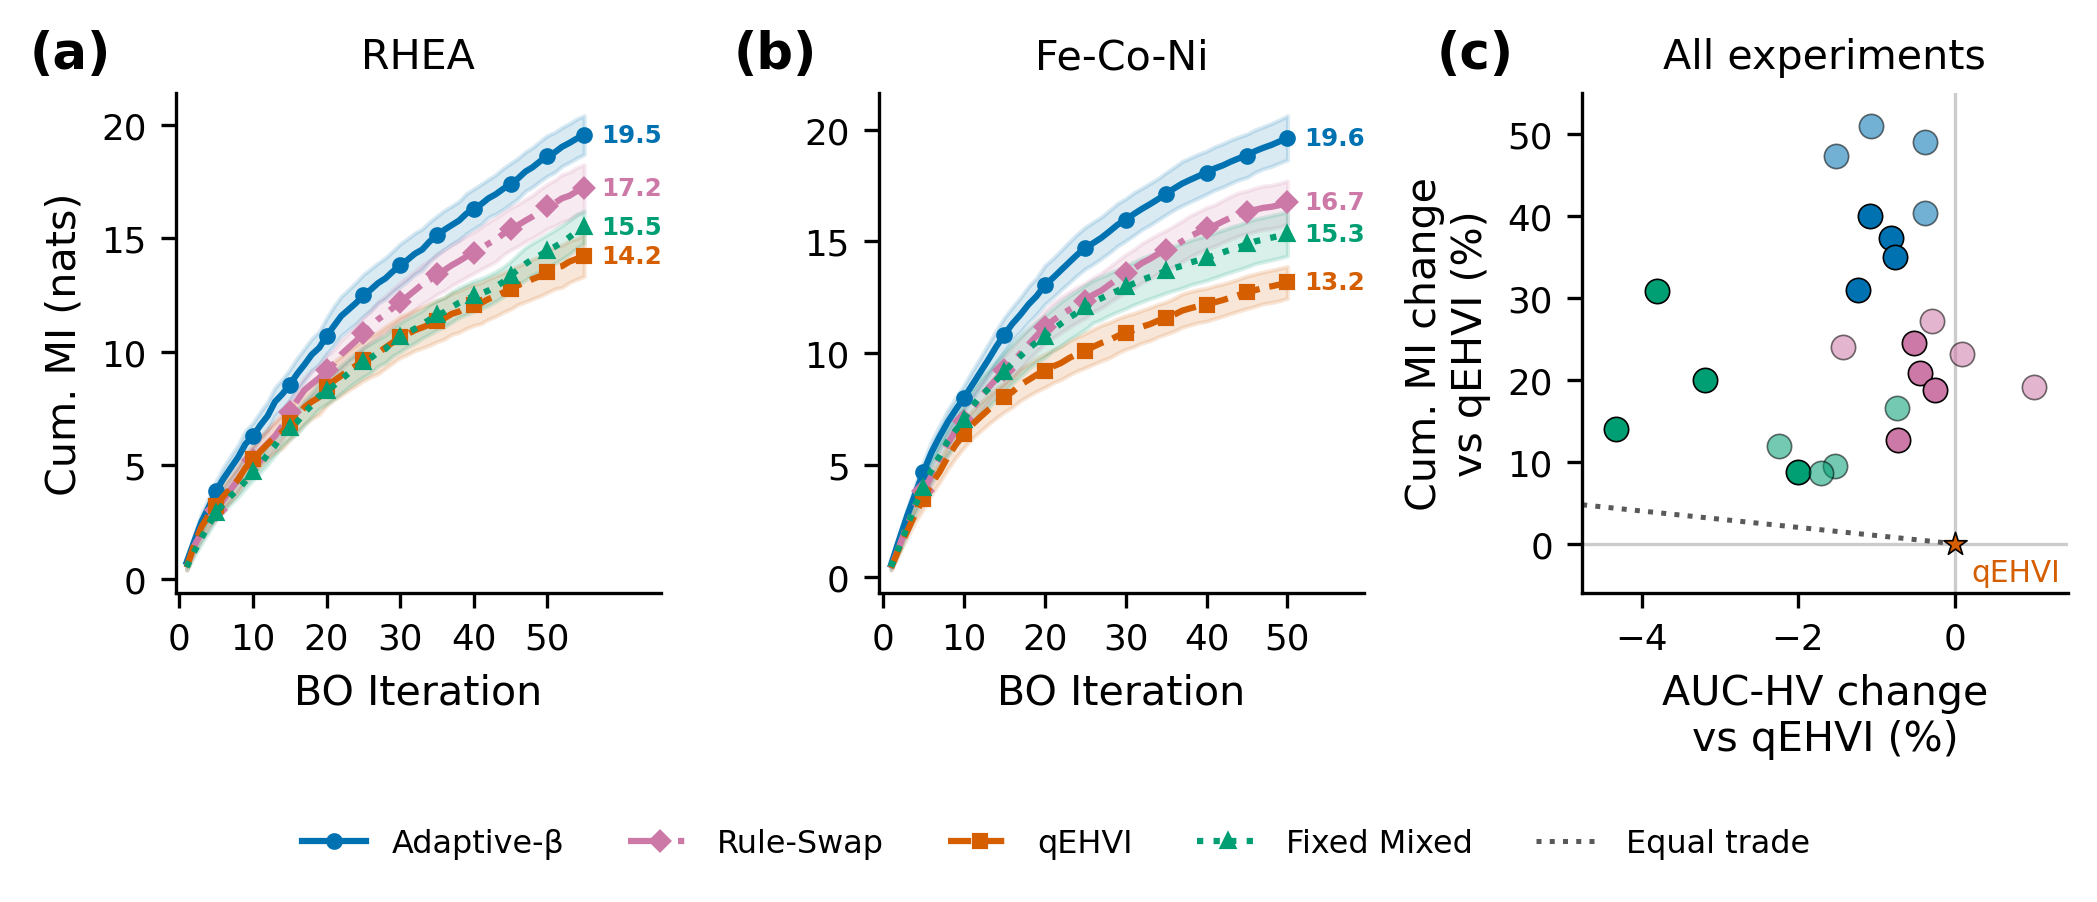
\includegraphics[width=\textwidth]{figures/fig5_mi_tradeoff.png}
    \caption{The information--optimization tradeoff across all eight experimental
             configurations ($n = 25$ seeds per strategy).
             \textbf{(a--b)} Cumulative mutual information over the baseline
             campaign for the RHEA and Fe-Co-Ni magnet systems; lines are
             per-strategy means and shaded bands are 95\% confidence intervals.
             \textbf{(c)} Cumulative MI gain plotted against AUC-HV cost, both
             expressed as a percentage change relative to the qEHVI baseline of
             the same experiment, which sits at the origin. Marker colour
             denotes strategy, and each experiment contributes one marker per
             mixed-allocation strategy; filled
             markers are the RHEA system and translucent markers the Fe-Co-Ni
             magnet system. The dotted line marks an equal trade, where the
             percentage of information gained equals the percentage of
             convergence speed given up. Every mixed-allocation point lies far
             above that line.
             End-of-campaign cumulative MI means are annotated at the
             right edge of (a) and (b); those values for all eight
             configurations, with their standard errors and alongside final
             hypervolume and AUC-HV, are tabulated in
             \ref{app:cumulative_mi_table}. Pairwise strategy
             comparisons reported anywhere in this work use the two-sided
             Wilcoxon signed-rank test on per-seed differences matched by
             shared random seed, with no multiple-comparison correction applied
             across the six strategy pairs within an experiment; the full
             matrix of $p$-values is given in
             \ref{app:significance}.}
    \label{fig:mi-tradeoff}
\end{figure}

In the RHEA system (Fig.~\ref{fig:baseline}, left column), all four strategies converged to nearly the same final hypervolume by the end of the 55-iteration baseline campaign. qEHVI reached the highest final hypervolume at $0.9983 \pm 0.00018$, followed by Fixed Mixed ($0.9971 \pm 0.00017$), Rule-Swap ($0.9970 \pm 0.00018$), and Adaptive-$\beta$ ($0.9967 \pm 0.00019$). Because the campaign was long enough for every strategy to approach the theoretical maximum, final hypervolume alone does not differentiate performance well. Examining how quickly each strategy accumulated the hypervolume over the course of the campaign reveals a clearer picture.
The area under the hypervolume curve (AUC-HV) showed a clear and consistent ordering in the RHEA system. qEHVI converged fastest at $52.02 \pm 0.08$, followed by Rule-Swap ($51.79 \pm 0.10$), Adaptive-$\beta$ ($51.59 \pm 0.09$), and Fixed Mixed ($50.98 \pm 0.09$). qEHVI, which allocates all resources toward exploitation of the predicted Pareto front, led throughout. The two adaptive strategies occupied the middle of the distribution, each accumulating roughly one fewer AUC unit than qEHVI over the 55-iteration campaign. Fixed Mixed fell furthest behind, reflecting its exploration-heavy early schedule that consistently delayed its ramp toward the high-performing region. This ordering follows how exploratory each strategy is early in the campaign, with greater early exploration yielding slower hypervolume accumulation.

The Fe-Co-Ni magnet system told a different story. The four strategies converged to mean final hypervolumes ranging from $0.84$ to $0.86$ over 50 iterations, with no statistically distinguishable differences between any strategy pair. AUC-HV values fell between $38.1$ and $38.4$ with no consistent ordering across strategies. The discontinuous Pareto front and larger design space likely drove the increased difficulty for all strategies. The near-identical outcomes across all strategies and seeds indicate that the Fe-Co-Ni magnet problem is simply very hard regardless of resource-allocation choice.

Mutual information separates the strategies where hypervolume does not. In both baseline campaigns, Adaptive-$\beta$ accumulated the most cumulative MI, followed by Rule-Swap, Fixed Mixed, and qEHVI; the per-configuration values for every experiment are given in Table~\ref{tab:cumulative-mi-full} and the baseline trajectories in Fig.~\ref{fig:mi-tradeoff}a--b. Adaptive-$\beta$ gained roughly $37\%$ more cumulative information than qEHVI over the 55 RHEA iterations and roughly $49\%$ more over the 50 Fe-Co-Ni magnet iterations. Its lead was established within the first ten iterations of both baseline campaigns and widened thereafter, so the separation is not an artifact of where a campaign happens to terminate.
% ---------------------------------------------------------------------------
\subsection{Optimization Performance Under Time and Budget Constraints}
\label{sec:results-events-hv}
% ---------------------------------------------------------------------------

\begin{figure}[htbp]
    \centering
    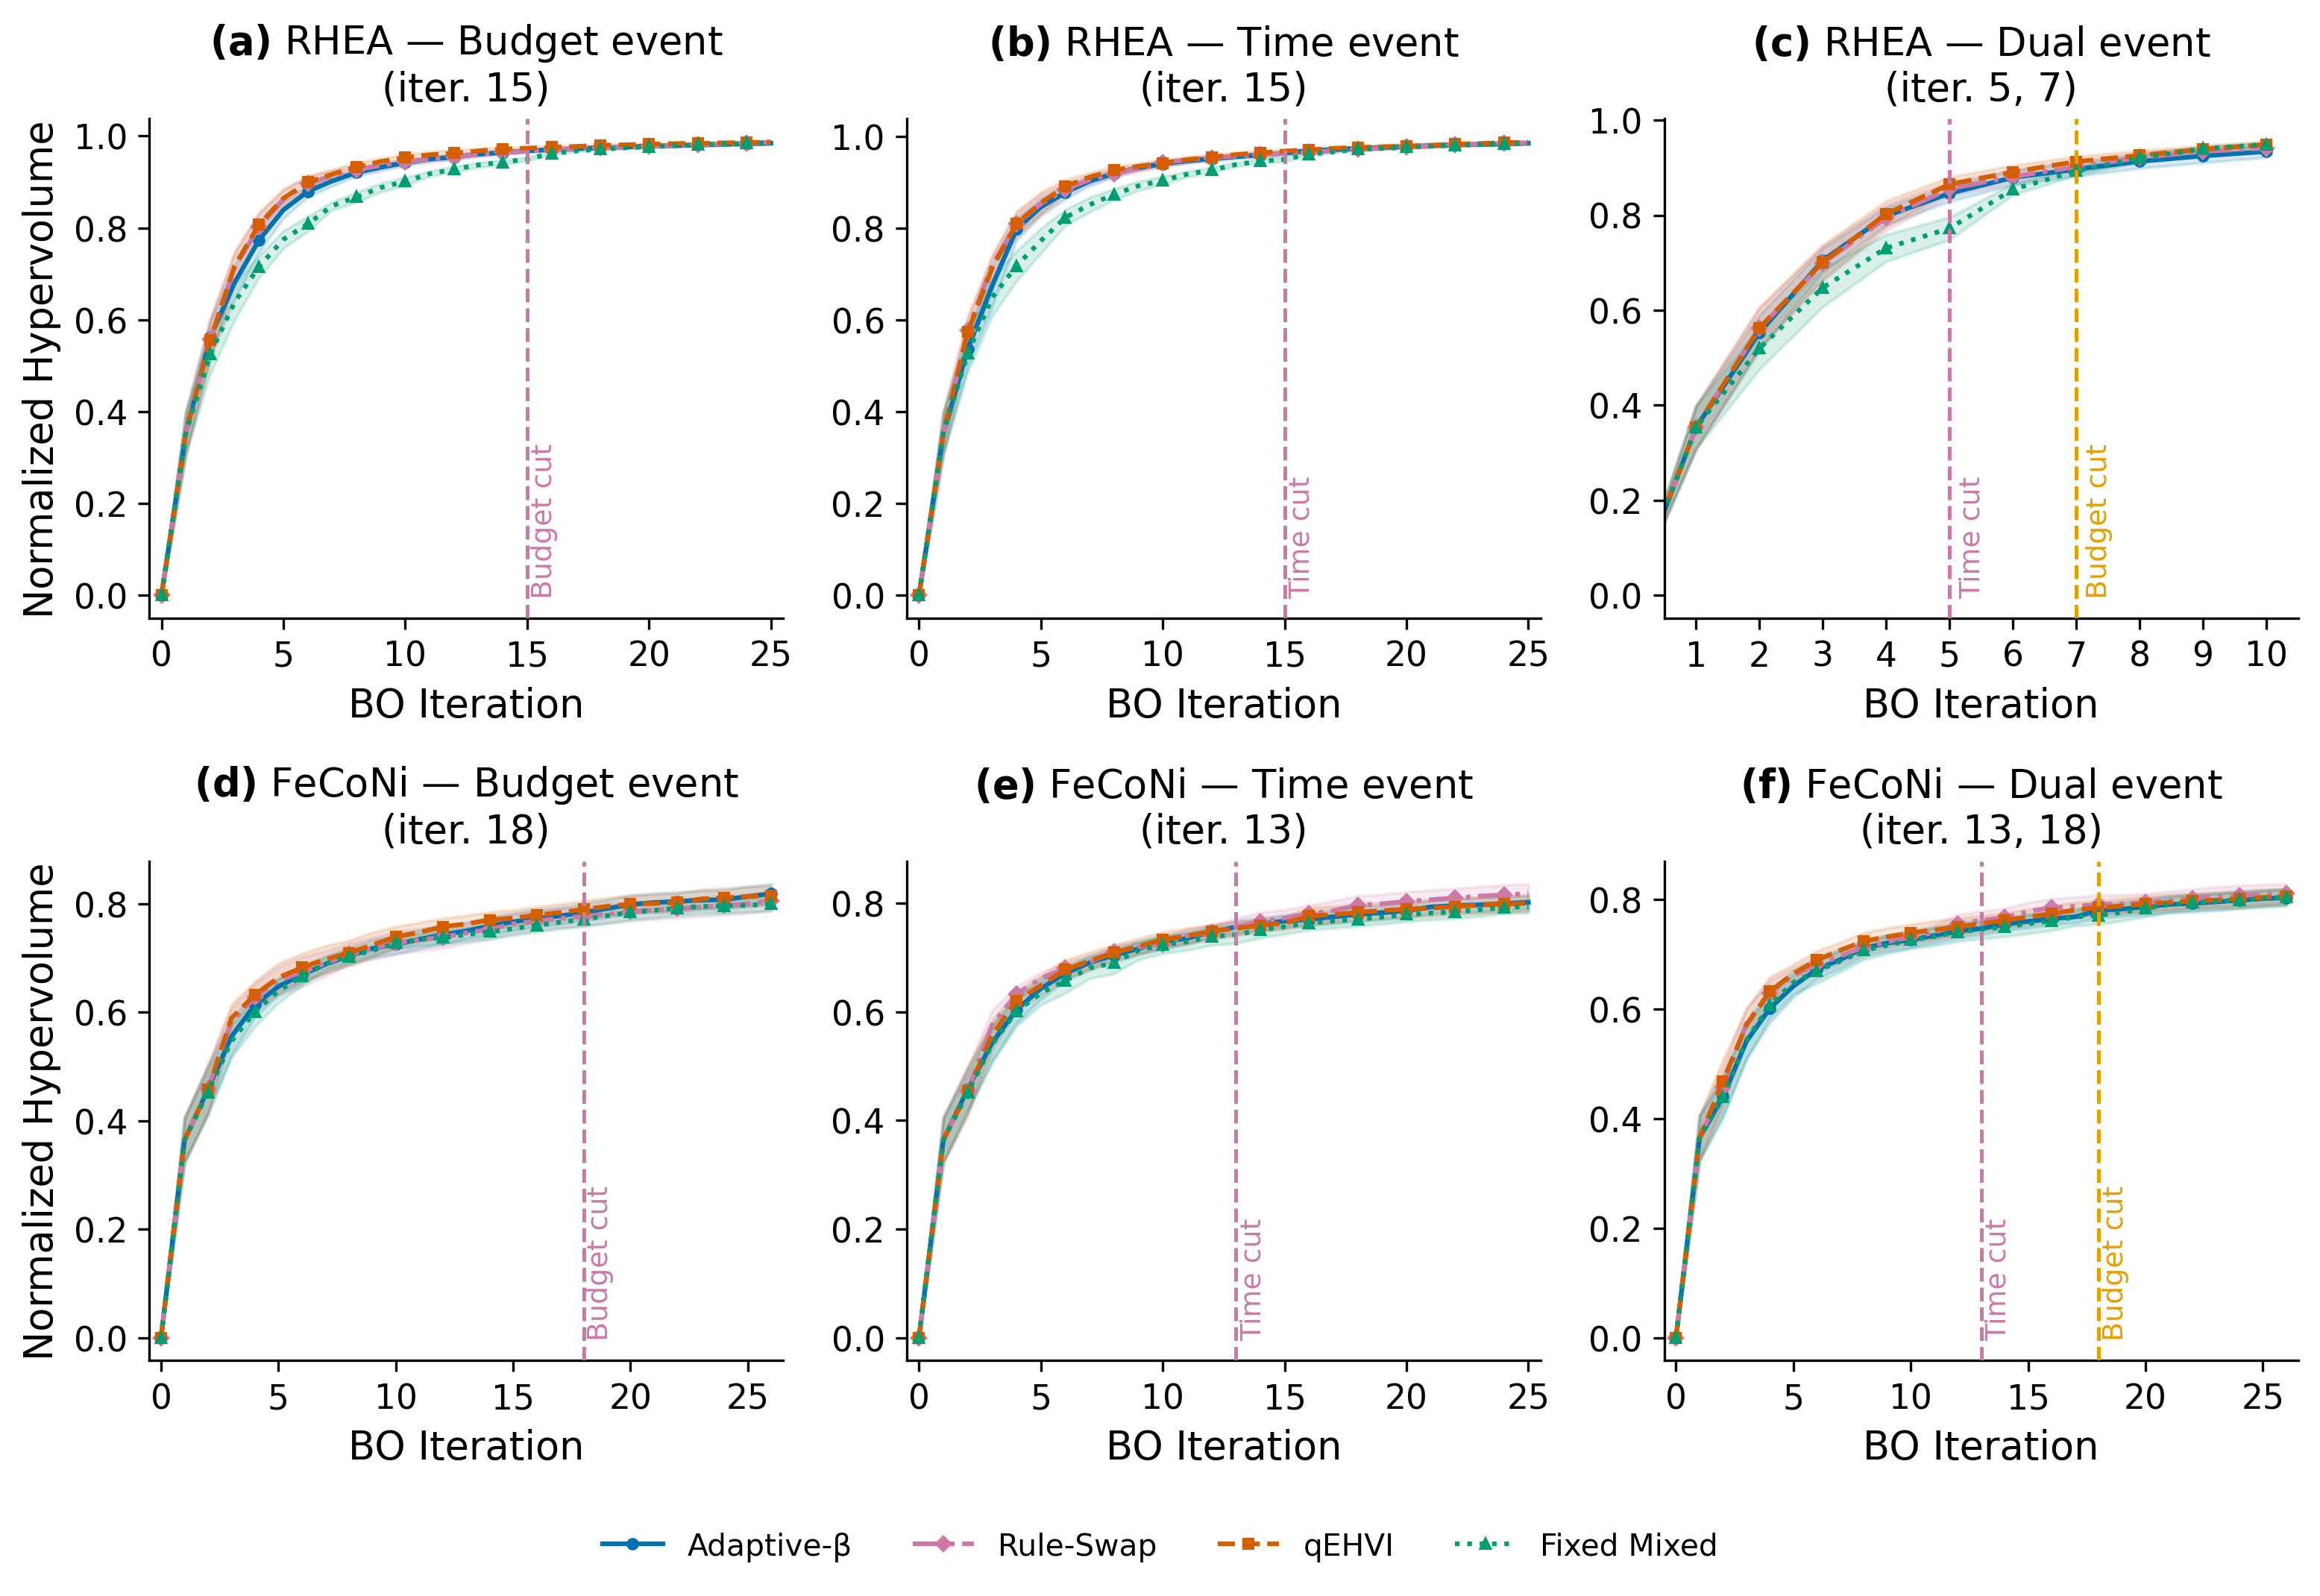
\includegraphics[width=\linewidth]{figures/fig6_event_hypervolume.png}
    \caption{Hypervolume convergence for all six event experiments.
             Mean $\pm$ 95\% confidence interval across $n = 25$ seeds.
             Dashed vertical lines mark the iteration(s) at which resource
             events were applied.
             \textbf{Top row}: RHEA system ($q = 5$).
             \textbf{Bottom row}: Fe-Co-Ni magnet system ($q = 5$).
             From left to right: budget-event, time-event, and dual-event configurations.
             Strategies: Adaptive-$\beta$ (blue), Rule-Swap (purple), qEHVI (orange), Fixed Mixed (green).}
    \label{fig:event_hv}
\end{figure}


Fig.~\ref{fig:event_hv} shows hypervolume trajectories across all six event experiments. Before any event was applied, Adaptive-$\beta$, Rule-Swap, and qEHVI entered the event phase with comparable hypervolume accumulation across all six experiments. Fixed Mixed consistently entered the RHEA event experiments with lower pre-event AUC-HV than the other three strategies, the same consequence of its exploration-heavy early schedule seen at baseline. Its exploration period had not yet finished converting into hypervolume gains.

In the RHEA budget and time events, the separation between strategies widened compared to baseline. qEHVI again led in final hypervolume, reaching $0.9869 \pm 0.00063$ in the budget event and $0.9866 \pm 0.00100$ in the time event. Adaptive-$\beta$ finished significantly below qEHVI in both cases ($0.9843 \pm 0.00071$ budget, $0.9848 \pm 0.00054$ time), a gap that was not present at baseline where the two strategies were indistinguishable in final hypervolume. Rule-Swap remained comparable to qEHVI in both events ($0.9861 \pm 0.00048$ and $0.9858 \pm 0.00044$), and Fixed Mixed fell significantly below qEHVI in both ($0.9855 \pm 0.00043$ and $0.9846 \pm 0.00054$). For AUC-HV, the baseline ordering held. qEHVI led ($22.11 \pm 0.08$ budget, $22.00 \pm 0.09$ time), with Adaptive-$\beta$ and Rule-Swap following, and Fixed Mixed significantly below all other strategies in both events. Mutual information again separated the strategies, with Adaptive-$\beta$ accumulating the most in both events ($12.29 \pm 0.38$ budget, $11.97 \pm 0.37$ time) and all three mixed-allocation strategies significantly exceeding qEHVI ($8.78 \pm 0.31$ budget, $8.86 \pm 0.39$ time). Rule-Swap and Fixed Mixed were not distinguishable from each other in either event; the full comparison is given in Table~\ref{tab:cumulative-mi-full} and Table~\ref{tab:significance}.
The RHEA dual event represented an extreme case of campaign compression, truncating the total campaign to only ten iterations. Under these conditions, the strategy ordering for final hypervolume changed considerably from baseline. Fixed Mixed and qEHVI finished with comparable final hypervolumes ($0.9488 \pm 0.00216$ and $0.9486 \pm 0.00318$ respectively), together at the top of the distribution. Rule-Swap also finished comparably to both ($0.9413 \pm 0.00423$). Adaptive-$\beta$ fell significantly below both qEHVI and Fixed Mixed, finishing at $0.9341 \pm 0.00602$, the largest hypervolume spread across strategies in any experiment at approximately $1.5\%$ of the theoretical maximum compared to under $0.2\%$ at baseline. For AUC-HV, qEHVI led ($7.43 \pm 0.07$), with Adaptive-$\beta$ ($7.33 \pm 0.07$) and Rule-Swap ($7.37 \pm 0.07$) following and comparable to each other, and Fixed Mixed significantly below all three ($7.10 \pm 0.07$). The MI separation compressed over the ten remaining iterations but Adaptive-$\beta$'s lead persisted, at $6.11 \pm 0.35$ nats against $4.66 \pm 0.33$ for qEHVI. Rule-Swap ($5.25 \pm 0.26$) and Fixed Mixed ($5.32 \pm 0.18$) finished between the two and were indistinguishable from each other, so the middle of the baseline ordering no longer resolved. Adaptive-$\beta$ remained significantly above both Rule-Swap and qEHVI, and Rule-Swap remained significantly above qEHVI.

The Fe-Co-Ni magnet system produced largely indistinguishable results across all four strategies in final hypervolume and AUC-HV for all three event types, consistent with the baseline result. Strategies finished the budget event campaigns between $0.80$ and $0.82$ normalized hypervolume, the time event between $0.79$ and $0.82$, and the dual event between $0.80$ and $0.81$, with no consistent ordering in any case. One exception is the budget event, where qEHVI led Fixed Mixed in AUC-HV at $18.46 \pm 0.18$ versus $18.05 \pm 0.13$, and Adaptive-$\beta$ finished with a slightly higher final hypervolume than Fixed Mixed ($0.8186 \pm 0.0088$ versus $0.7992 \pm 0.0063$). In the time event, Rule-Swap led Fixed Mixed in AUC-HV at $17.62 \pm 0.12$ versus $17.17 \pm 0.16$. Mutual information across all three Fe-Co-Ni magnet event experiments followed the same ordering seen at baseline, with Adaptive-$\beta$ leading, Rule-Swap second, and both strategies accumulating substantially more MI than qEHVI.

% ---------------------------------------------------------------------------
\subsection{Convergence to Milestone Hypervolume Thresholds}
\label{sec:results-convergence}
% ---------------------------------------------------------------------------

\begin{table*}[]
\centering
\small
\setlength{\tabcolsep}{5pt}
\begin{tabular}{@{}lllccc@{}}
\toprule
\multirow{2}{*}{System} & \multirow{2}{*}{Experiment} & \multirow{2}{*}{Strategy}
  & \multicolumn{1}{c}{Batches to 50\% HV}
  & \multicolumn{2}{c}{Batches to 80\% HV} \\
\cmidrule(l){5-6}
 & & & Mean $\pm$ 95\% CI & Mean $\pm$ 95\% CI & \% reached \\
\midrule
  \multirow{16}{*}{Fe-Co-Ni} & \multirow{4}{*}{Baseline} & Adaptive-$\beta$ & $2.7 \pm 0.4$ & $29.7 \pm 4.6$ & 96\% \\
   &  & Rule-Swap & $2.5 \pm 0.4$ & $27.4 \pm 4.1$ & 92\% \\
   &  & qEHVI & $2.4 \pm 0.3$ & $26.3 \pm 4.2$ & 96\% \\
   &  & Fixed Mixed & $2.9 \pm 0.6$ & $28.3 \pm 3.9$ & 96\% \\
  \addlinespace[2pt]
   & \multirow{4}{*}{Budget event} & Adaptive-$\beta$ & $2.6 \pm 0.4$ & $20.1 \pm 2.5$ & 64\% \\
   &  & Rule-Swap & $2.6 \pm 0.5$ & $18.7 \pm 5.2$ & 40\% \\
   &  & qEHVI & $2.6 \pm 0.6$ & $18.6 \pm 4.4$ & 52\% \\
   &  & Fixed Mixed & $2.9 \pm 0.5$ & $20.0 \pm 3.6$ & 36\% \\
  \addlinespace[2pt]
   & \multirow{4}{*}{Time event} & Adaptive-$\beta$ & $2.8 \pm 0.5$ & $17.7 \pm 5.3$ & 28\% \\
   &  & Rule-Swap & $2.5 \pm 0.3$ & $17.5 \pm 3.3$ & 44\% \\
   &  & qEHVI & $2.6 \pm 0.4$ & $16.1 \pm 4.2$ & 32\% \\
   &  & Fixed Mixed & $3.0 \pm 0.5$ & $20.6 \pm 4.5$ & 32\% \\
  \addlinespace[2pt]
   & \multirow{4}{*}{Dual event} & Adaptive-$\beta$ & $2.9 \pm 0.5$ & $19.8 \pm 4.9$ & 36\% \\
   &  & Rule-Swap & $2.6 \pm 0.4$ & $16.6 \pm 3.7$ & 44\% \\
   &  & qEHVI & $2.7 \pm 0.4$ & $19.6 \pm 3.7$ & 52\% \\
   &  & Fixed Mixed & $2.9 \pm 0.5$ & $19.5 \pm 3.6$ & 52\% \\
\midrule
\multicolumn{4}{@{}l}{} & \multicolumn{2}{c}{Batches to 90\% HV} \\[-4pt]
\cmidrule(l){5-6}
  \multirow{16}{*}{RHEA} & \multirow{4}{*}{Baseline} & Adaptive-$\beta$ & $2.3 \pm 0.4$ & $7.4 \pm 0.6$ & 100\% \\
   &  & Rule-Swap & $2.2 \pm 0.3$ & $6.8 \pm 0.5$ & 100\% \\
   &  & qEHVI & $2.2 \pm 0.3$ & $6.2 \pm 0.5$ & 100\% \\
   &  & Fixed Mixed & $2.2 \pm 0.3$ & $9.8 \pm 0.6$ & 100\% \\
  \addlinespace[2pt]
   & \multirow{4}{*}{Budget event} & Adaptive-$\beta$ & $2.1 \pm 0.3$ & $7.3 \pm 0.5$ & 100\% \\
   &  & Rule-Swap & $2.1 \pm 0.3$ & $6.6 \pm 0.7$ & 100\% \\
   &  & qEHVI & $2.1 \pm 0.3$ & $6.6 \pm 0.7$ & 100\% \\
   &  & Fixed Mixed & $2.3 \pm 0.4$ & $10.1 \pm 0.5$ & 100\% \\
  \addlinespace[2pt]
   & \multirow{4}{*}{Time event} & Adaptive-$\beta$ & $2.4 \pm 0.4$ & $7.4 \pm 0.5$ & 100\% \\
   &  & Rule-Swap & $2.0 \pm 0.2$ & $7.0 \pm 0.6$ & 100\% \\
   &  & qEHVI & $2.0 \pm 0.2$ & $6.8 \pm 0.6$ & 100\% \\
   &  & Fixed Mixed & $2.2 \pm 0.3$ & $9.9 \pm 0.6$ & 100\% \\
  \addlinespace[2pt]
   & \multirow{4}{*}{Dual event} & Adaptive-$\beta$ & $2.2 \pm 0.3$ & $7.2 \pm 0.6$ & 88\% \\
   &  & Rule-Swap & $2.2 \pm 0.3$ & $7.2 \pm 0.5$ & 96\% \\
   &  & qEHVI & $2.2 \pm 0.3$ & $6.8 \pm 0.6$ & 100\% \\
   &  & Fixed Mixed & $2.4 \pm 0.4$ & $7.8 \pm 0.2$ & 100\% \\
\bottomrule
\end{tabular}
\caption{Batches required to reach 50\% and the upper milestone hypervolume threshold (mean $\pm$ 95\% CI; $n = 25$ seeds per strategy). All seeds reach the 50\% milestone in every experiment. Upper milestone thresholds differ by system, 80\% for the Fe-Co-Ni magnet problem; 90\% for the RHEA problem. The \% column reports the fraction of seeds reaching the upper milestone.}
\label{tab:convergence-speed}
\end{table*}

All four strategies reached the 50\% hypervolume milestone reliably in both systems and across every experiment. In the RHEA system, mean batch counts to the 50\% milestone were nearly identical across strategies and experiments, ranging from 2.0 to 2.4 batches, with all seeds reaching the threshold in every case. The 50\% threshold is reached early enough in RHEA campaigns that strategy choice has no meaningful effect on when it is first crossed. The Fe-Co-Ni magnet system required slightly more time at 2.4 to 3.0 mean batches at baseline, with Fixed Mixed taking about 0.5 more batches than qEHVI due to its exploration-heavy opening. Resource events shifted these early-campaign timings only negligibly in either system.

The 90\% milestone in the RHEA system revealed a clear and consistent ordering across the baseline, budget, and time event experiments. qEHVI reached the threshold fastest, averaging $6.2 \pm 0.5$, $6.6 \pm 0.7$, and $6.8 \pm 0.6$ batches in the baseline, budget, and time experiments respectively, all at 100\% seed coverage. Rule-Swap followed at $6.8 \pm 0.5$, $6.6 \pm 0.7$, and $7.0 \pm 0.6$ batches, and Adaptive-$\beta$ at $7.4 \pm 0.6$, $7.3 \pm 0.5$, and $7.4 \pm 0.5$ batches, both at 100\% coverage. Fixed Mixed was consistently the slowest at $9.8 \pm 0.6$, $10.1 \pm 0.5$, and $9.9 \pm 0.6$ batches, roughly 3--4 more than qEHVI in every case, reflecting the extended early exploration phase that delays its ramp toward the high-performing region. This ordering mirrors the AUC-HV pattern from Section~\ref{sec:results-baseline}, and budget and time events did not disrupt it.

The dual event was the one exception in the RHEA system. Fixed Mixed dropped from $9.8 \pm 0.6$ batches at baseline to $7.8 \pm 0.2$ batches at 100\% seed coverage, closing most of the gap to the other strategies. The dual event compressed the extended early exploration phase that normally slows Fixed Mixed down, forcing it into exploitation sooner. Adaptive-$\beta$ required $7.2 \pm 0.6$ batches at 88\% seed coverage, Rule-Swap $7.2 \pm 0.5$ batches at 96\% coverage, and qEHVI $6.8 \pm 0.6$ batches at 100\% coverage, all modest shifts within one batch of their baseline values. Notably, Adaptive-$\beta$'s coverage dropped to 88\%, meaning 3 of 25 seeds failed to reach the 90\% threshold within the compressed dual-event campaign.

The Fe-Co-Ni magnet system shows a different picture driven by problem difficulty. At baseline, all strategies reached the 80\% milestone in 92--96\% of seeds, with mean batch counts of 26.3 to 29.7 out of 50 total batches, meaning the upper milestone typically required more than half the entire campaign budget to reach. In budget events, coverage fell to 36--64\% in all strategies, with Adaptive-$\beta$ maintaining the highest coverage at 64\%, followed by qEHVI (52\%), Rule-Swap (40\%) and Fixed Mixed (36\%). Time events were more damaging, with coverage ranging from 28--44\% and no consistent ordering. Dual events produced similar coverage of 36--52\%, with qEHVI and Fixed Mixed both reaching 52\%. The combination of a large and fragmented design space with event-driven campaign truncation largely prevented strategies from reaching the upper hypervolume threshold in the Fe-Co-Ni magnet problem, making milestone comparisons between strategies unreliable under event conditions.

% ---------------------------------------------------------------------------
\subsection{\texorpdfstring{$\beta$}{β} Coefficient Trajectories Under Baseline and Event Conditions}
\label{sec:results-beta}
% ---------------------------------------------------------------------------

\begin{figure}[htbp]
    \centering
    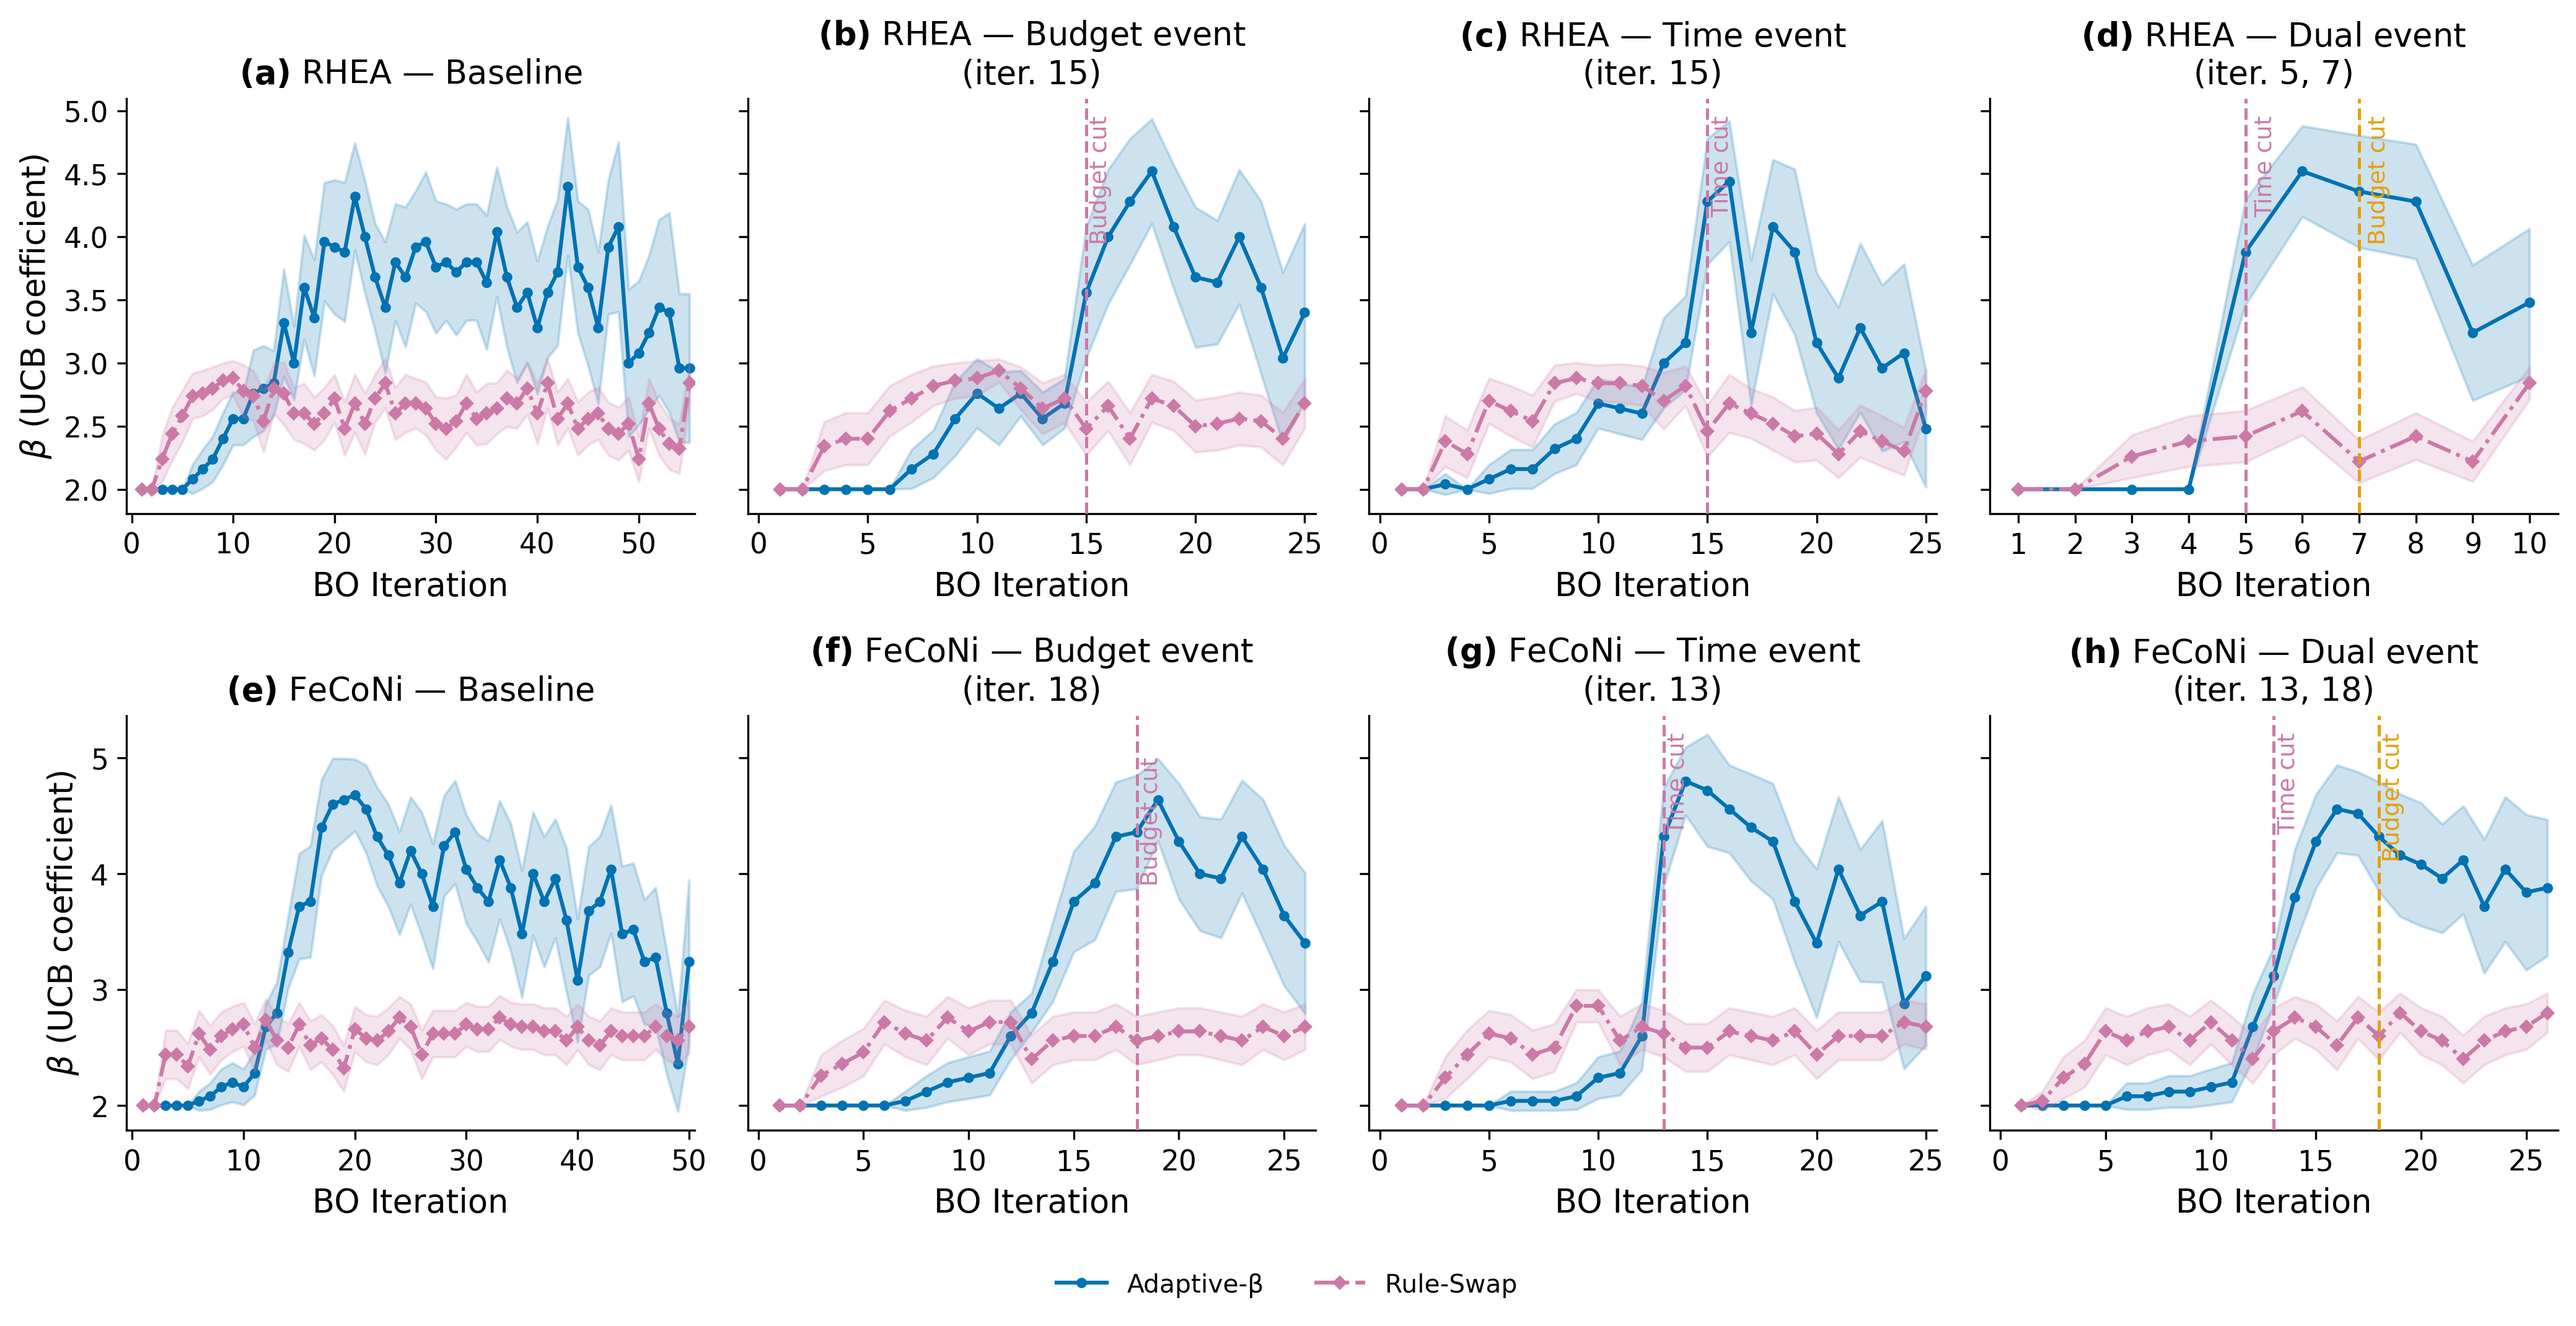
\includegraphics[width=\textwidth]{figures/fig7_beta_trajectories.png}
    \caption{Adaptive-$\beta$ (blue, circles) and Rule-Swap (purple, diamonds) $\beta$ selection
             across all eight experimental configurations ($n = 25$ seeds per strategy).
             \textbf{Top row (a--d)}: RHEA system.
             \textbf{Bottom row (e--h)}: Fe-Co-Ni magnet system.
             Columns from left to right show the baseline, budget cut, time cut, and time-plus-budget cut configurations.
             Lines show per-seed means; shaded bands are 95\% confidence intervals.
             Dashed vertical lines mark the iterations at which resource events were applied.
             The dotted horizontal line marks $\beta = 2.0$, the minimum selectable value.}
    \label{fig:beta}
\end{figure}

The previous sections established how the strategies performed in terms of optimization outcomes. This section examines what the two LLM-based strategies were actually doing internally, specifically how Adaptive-$\beta$ and Rule-Swap set their parameters across the campaign and in response to events, in order to characterize whether their decision-making followed the intended design and what patterns emerged across problems.
At baseline, Rule-Swap's $\beta$ selections held within a narrow band centered near 2.5, spanning 2.0 to 3.5 without any directional trend in either system. This is consistent with the design of the rule shift, where $\beta$ is a secondary parameter, and the primary lever is the number of exploration candidates per batch. Adaptive-$\beta$ used $\beta$ as its main control mechanism and followed a very different trajectory. In the RHEA system, $\beta$ rose sharply from $2.14 \pm 0.03$ in early iterations (1--10) to $3.53 \pm 0.06$ in the middle phase (11--30), peaking near iteration 20, before plateauing through the final phase at $3.57 \pm 0.07$ (31--55). The Fe-Co-Ni magnet system followed a similar pattern, rising from $2.06 \pm 0.02$ in early iterations to $3.92 \pm 0.07$ in the middle phase before declining modestly to $3.55 \pm 0.08$ in the final phase. Both strategies became less exploratory as the campaign progressed, with Adaptive-$\beta$ doing so by ramping $\beta$ toward higher-variance candidate selection while gradually reducing exploration slots, and Rule-Swap by reducing its exploration candidate count toward zero in the final iterations of both baseline campaigns.

Looking at the within-campaign $\beta$ trajectory for Adaptive-$\beta$ in Fig.~\ref{fig:beta}, the ramp in the RHEA system is not smooth. The agent tended to make a large adjustment to $\beta$ and then hold for several iterations of smaller, stabilizing changes before making another large move, producing a step-like pattern. This is consistent with an agent that adjusts $\beta$ substantially, observes the effect on the noisy MI signal over a few iterations, and then re-adjusts. Given how much the per-iteration MI values fluctuate, as visible in Fig.~\ref{fig:baseline}, this test-and-adjust pattern is a plausible response to a feedback channel with high iteration-to-iteration variance.

Under event conditions, both strategies showed trends that were consistent with their baseline behavior, with the primary difference being timing. In the RHEA budget and time experiments, Adaptive-$\beta$'s post-event $\beta$ values were comparable to the baseline trajectory at the same iteration numbers, suggesting that the event advanced the campaign clock rather than triggering fundamentally new behavior. This was true regardless of whether the constraint was framed as a budget reduction or a time cut, indicating that the strategy response $\beta$ depended on the remaining iterations rather than the specific nature of the constraint. The RHEA dual experiment was the exception, where post-event $\beta$ significantly exceeded the baseline trajectory at those early iteration numbers, pointing to a genuine urgency response under extreme compression. In the Fe-Co-Ni magnet system, post-event $\beta$ matched the baseline trajectory across all three event types, mirroring the flat mid-to-late $\beta$ behavior seen at baseline. Rule-Swap's $\beta$ showed no consistent directional change under any event condition, and its primary behavioral response to events was in allocation, which is discussed in Section~\ref{sec:results-events-behavior}.

% ---------------------------------------------------------------------------
\subsection{Constraint Influence on Decision Making}
\label{sec:results-events-behavior}
% ---------------------------------------------------------------------------

\begin{figure}[htbp]
    \centering
    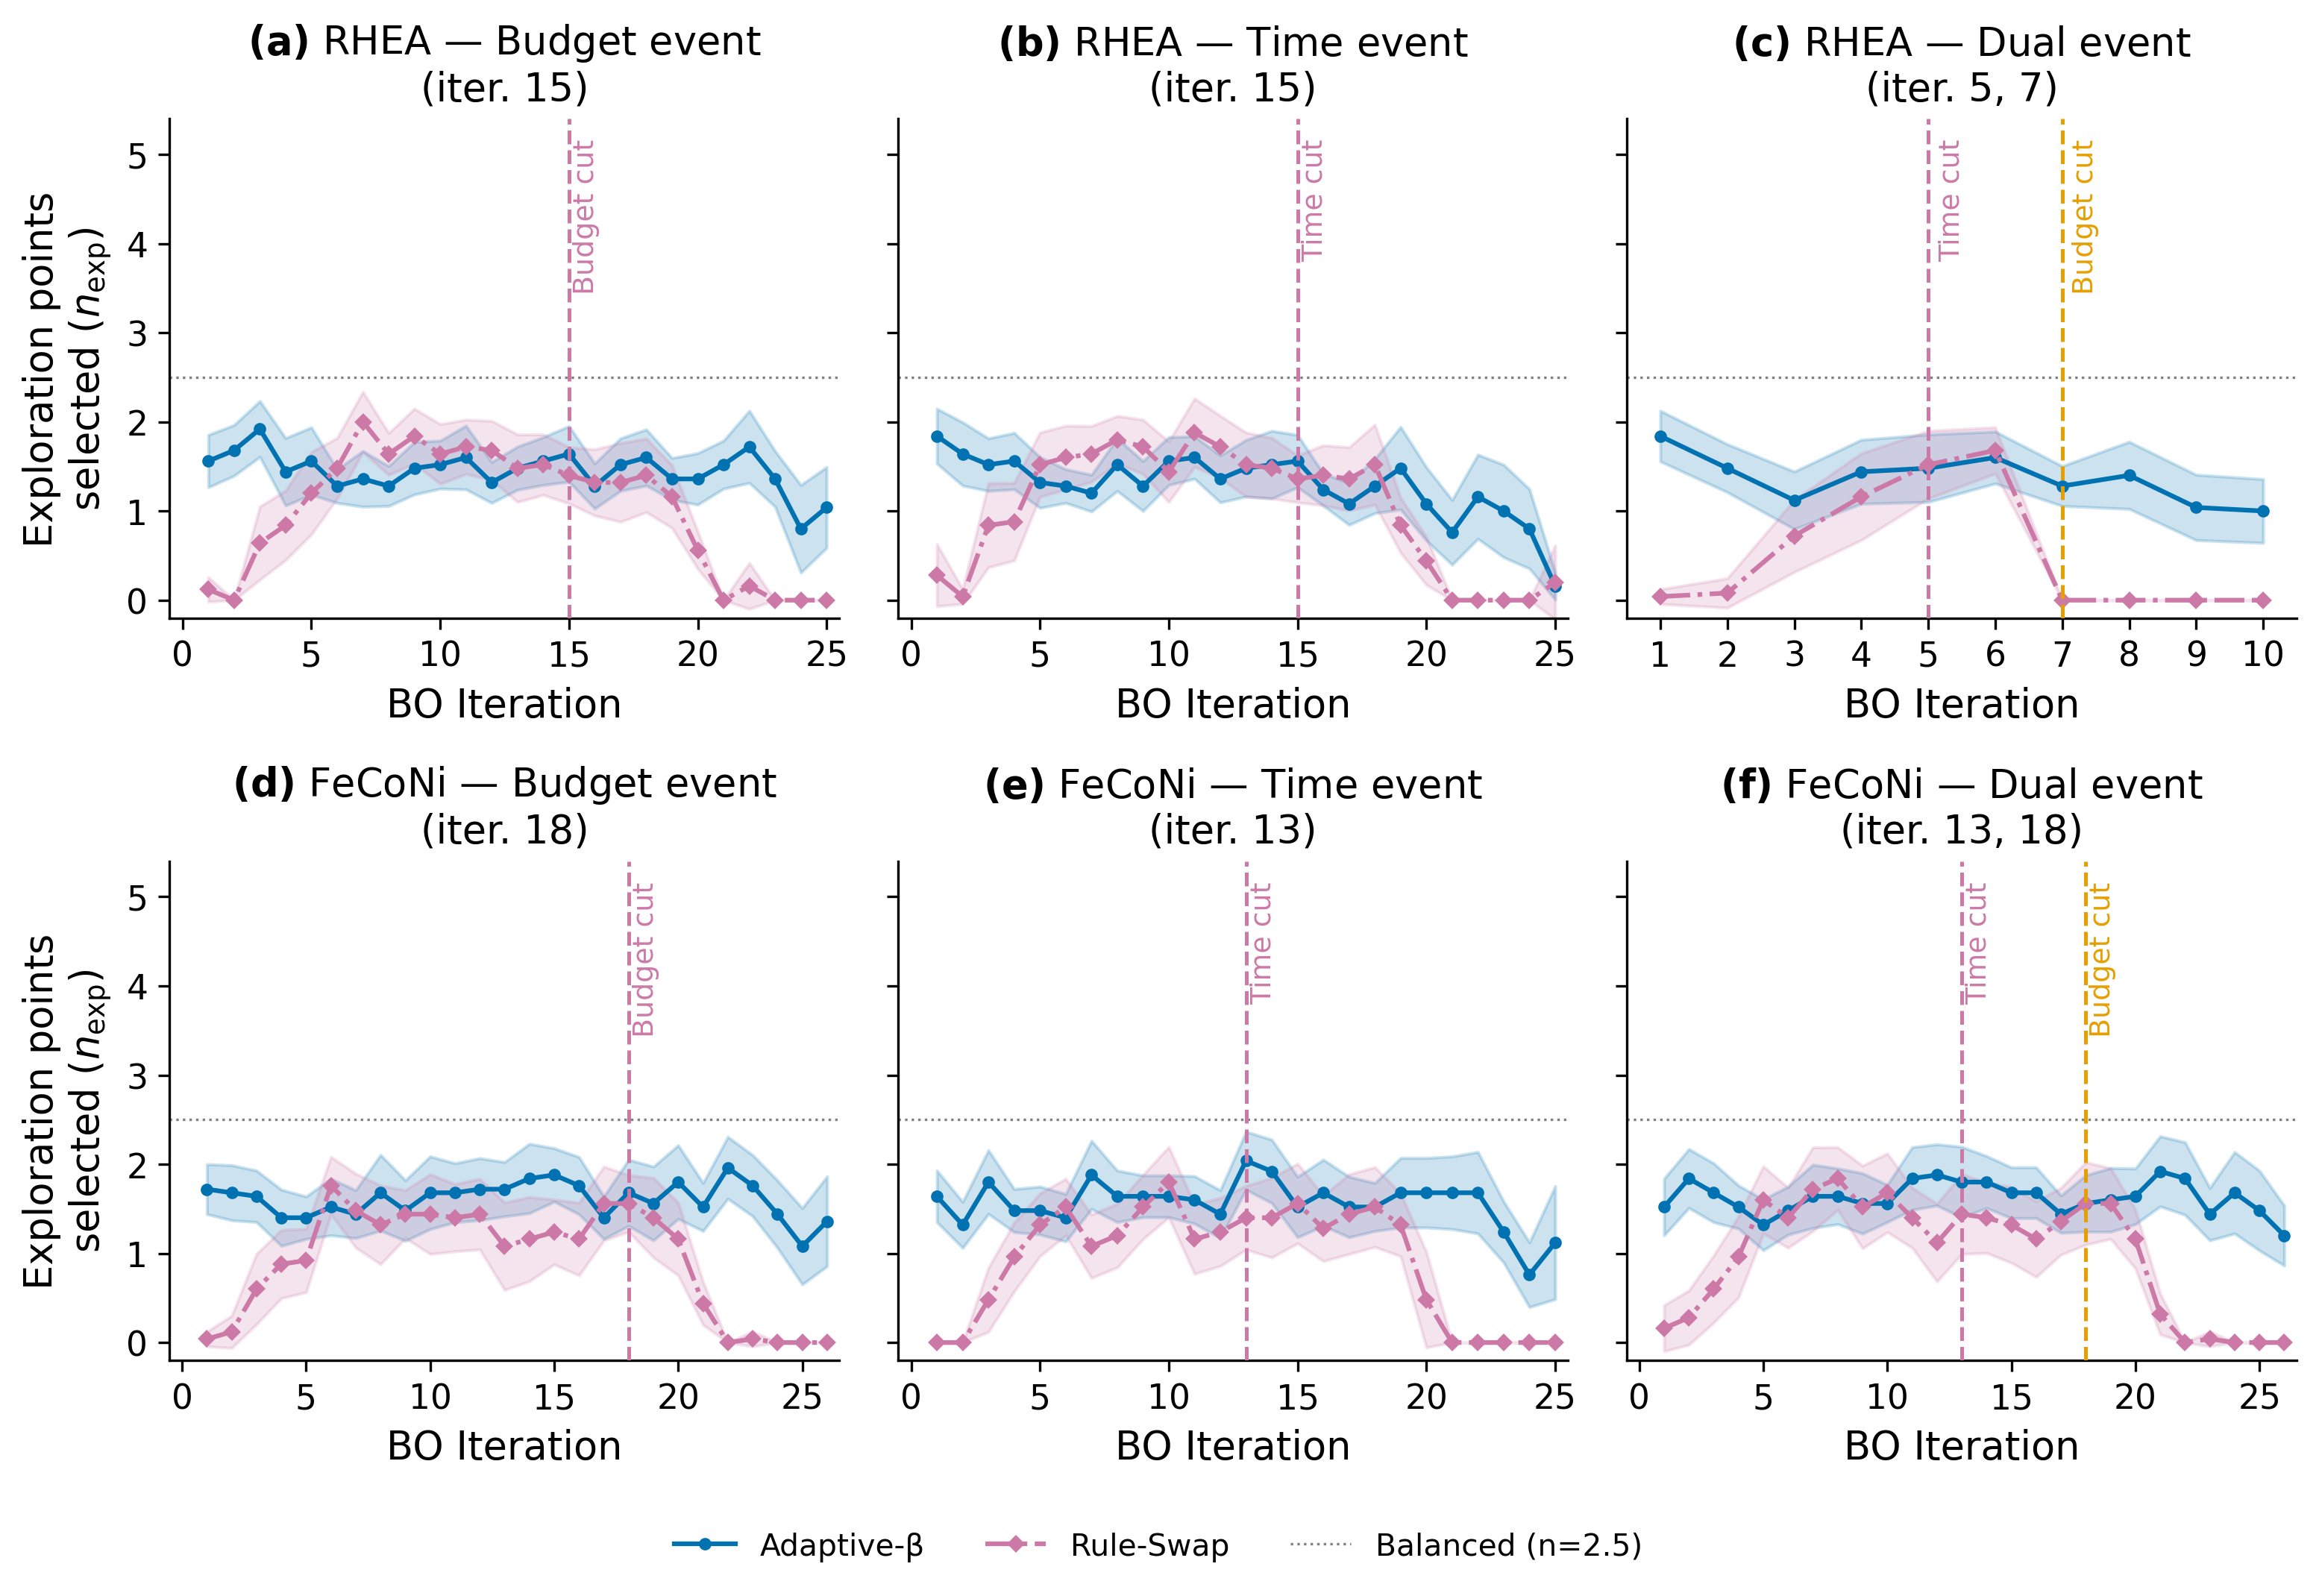
\includegraphics[width=\textwidth]{figures/fig8_event_allocation.png}
    \caption{Exploration candidate allocation ($n_\mathrm{exp}$) for Adaptive-$\beta$ and Rule-Swap across all six
             event experiments.
             Mean across $n = 25$ seeds; shaded bands are 95\% confidence
             intervals. Dashed vertical lines mark the iteration at which
             each resource event was applied; colors distinguish event type
             (pink: first event; orange: second event in dual-event
             experiments).
             The dotted horizontal line marks the balanced allocation.
             \textbf{Top row}: RHEA system.
             \textbf{Bottom row}: Fe-Co-Ni magnet system.
             From left to right: budget-event, time-event, and dual-event configurations.}
    \label{fig:event_alloc}
\end{figure}

Fig.~\ref{fig:event_alloc} shows how Adaptive-$\beta$ and Rule-Swap adjusted their exploration candidate allocation ($n_\mathrm{exp}$) across all six event experiments. For Rule-Swap, $n_\mathrm{exp}$ was the primary mechanism through which the agent controlled resource allocation. Understanding how it changed with events therefore speaks directly to whether the strategy behaved as intended.
At baseline, both strategies selected approximately 1.5 exploration candidates per batch for most of the campaign in both systems. Rule-Swap gradually reduced $n_\mathrm{exp}$ toward zero in the final iterations of both baseline campaigns, consistent with its end-of-campaign shift toward exploitation. Adaptive-$\beta$ showed a similarly slight downward trend over time, generally maintaining at least one exploration candidate per batch throughout.

Under event conditions in the RHEA system, Rule-Swap's allocation response was immediate and large. In the budget event, post-event $n_\mathrm{exp}$ dropped to $0.59 \pm 0.06$ candidates per batch, compared to $1.37 \pm 0.04$ at the same baseline iterations, a reduction of $0.78$ candidates per batch. The time event produced a comparable reduction, with post-event $n_\mathrm{exp}$ of $0.58 \pm 0.05$ against a baseline of $1.37 \pm 0.04$, a drop of $0.79$ per batch. In the RHEA dual event, Rule-Swap's post-event $n_\mathrm{exp}$ reached zero and remained there for every remaining iteration.
Adaptive-$\beta$'s RHEA allocation response was substantially smaller and differed between event types. In the budget event, post-event $n_\mathrm{exp}$ was $1.36 \pm 0.06$, essentially unchanged from the $1.35 \pm 0.03$ at the baseline at the same iterations. The time event produced a larger reduction, with post-event $n_\mathrm{exp}$ dropping to $1.00 \pm 0.09$ from a baseline of $1.35 \pm 0.03$, a reduction of roughly $0.35$ candidates per batch. The dual event showed a modest but significant reduction from $1.36 \pm 0.03$ to $1.15 \pm 0.12$. Adaptive-$\beta$ treated a time constraint as a more direct reason to reduce exploration candidates than a budget constraint, suggesting that the framing of the constraint influenced the agent's allocation decisions differently even when both event types produced comparable $\beta$ responses.

In the Fe-Co-Ni magnet system, Rule-Swap again reduced $n_\mathrm{exp}$ significantly after each event type, dropping from $1.12 \pm 0.05$ to $0.38 \pm 0.05$ in the budget event, from $1.02 \pm 0.03$ to $0.75 \pm 0.06$ in the time event, and from $1.19 \pm 0.05$ to $0.39 \pm 0.04$ in the dual event, all relative to a baseline near $1.26$ at the same iterations. Adaptive-$\beta$ showed no significant change in $n_\mathrm{exp}$ after any of the three Fe-Co-Ni magnet event experiments, maintaining post-event allocations near $1.56$--$1.60$ candidates per batch, comparable to the baseline trajectory throughout. Rather than adjusting candidate counts in response to events, Adaptive-$\beta$'s primary adjustment mechanism in the Fe-Co-Ni magnet system was $\beta$, or in this case the absence of a $\beta$ response, as described in Section~\ref{sec:results-beta}. Across both systems and all event types, the two strategies responded to resource constraints through opposite mechanisms. Rule-Swap reduced exploration candidates consistently and aggressively, while Adaptive-$\beta$ held allocation steady and relied on $\beta$ as the primary adjustment lever.

\section{Discussion}
\label{sec:discussion}

In this work, with the set of experiments investigates, we show that the primary differences between resource allocation strategies lay in mutual information accumulated and convergence speed rather than final hypervolume, consistent across both alloy systems. No mixed-allocation strategy outperformed qEHVI for final hypervolume or AUC-HV, yet all three exceeded qEHVI substantially in cumulative MI. Fig.~\ref{fig:mi-tradeoff}c makes that tradeoff comparable across all eight configurations by expressing each mixed strategy as a percentage change against the qEHVI baseline of its own experiment, which removes the differing hypervolume and MI scales of the two systems. All twenty-four mixed-allocation points lie above the equal-trade line, where the percentage of information gained would equal the percentage of convergence speed given up, and they lie well above it: the median ratio of proportional information gained to proportional AUC-HV given up is roughly $28$, with no configuration below $3$. Adaptive-$\beta$ sits furthest into that region in both systems, and the Fe-Co-Ni magnet configurations cluster near the vertical axis, where the AUC-HV cost is small and, in all but one comparison, not statistically resolvable. The annotated baseline curves in Fig.~\ref{fig:mi-tradeoff}a--b and the full values in Table~\ref{tab:cumulative-mi-full} show the same qualitative ordering: Adaptive-$\beta$ accumulated the most cumulative MI, qEHVI the least, and Rule-Swap and Fixed Mixed fell between them. All four strategies produced statistically indistinguishable final hypervolumes on the Fe-Co-Ni magnet problem, making cumulative MI and AUC-HV the only metrics by which strategies could be meaningfully compared there.

The mixed-allocation strategies traded AUC-HV and convergence speed for greater uncertainty reduction around the Pareto front at each iteration. The greater MI gains suggested that the GP surrogate was likely better characterized in the Pareto-front neighborhood for exploration-biased campaigns than for purely exploitative ones, as higher MI per iteration reflected the acquisition of more informative measurements relative to the current surrogate uncertainty about the Pareto front. Whether that improved characterization translated into practically meaningful outcomes for downstream materials analysis, such as more informative experimental records for objective refinement or follow-on campaigns, was not directly measured here and remains an open question.

Whether this tradeoff favors an adaptive policy over a fixed mixed schedule is what the resource-constraint experiments reveal. Resource events did not substantially change per-iteration optimization performance for any strategy relative to the baseline at the same point in the campaign, as reflected in the milestone convergence data of Table~\ref{tab:convergence-speed}, where batch counts to the 90\% hypervolume threshold fell within one batch of baseline values for all budget and time events. The primary effect of events was to reveal differences in how strategies compared to one another over a shortened campaign. HV performance in the Fe-Co-Ni magnet problem was largely indistinguishable across strategies under single events. The budget event yielded two exceptions: Adaptive-$\beta$ finished above Fixed Mixed in final hypervolume ($0.8186 \pm 0.0088$ versus $0.7992 \pm 0.0063$, $p = 0.045$), and qEHVI led Fixed Mixed in AUC-HV ($18.46 \pm 0.18$ versus $18.05 \pm 0.13$, $p = 0.026$). In the time event, Rule-Swap also led Fixed Mixed in AUC-HV ($17.62 \pm 0.12$ versus $17.17 \pm 0.16$, $p = 0.027$). All other pairings remained statistically indistinguishable. 

However, the RHEA experiments showed a clearer effect of the shortened campaign. qEHVI required no behavioral response because it already allocated all resources to exploitation, and Rule-Swap compressed its end-of-campaign exploration allocation in response, while Adaptive-$\beta$'s allocation remained near baseline under the budget constraint and reduced more substantially under the time constraint. Fixed Mixed however could not adapt the mixed allocation according to the shortened campaign, causing the AUC-HV gap relative to the other three strategies to widen across all three RHEA event types compared to baseline, visible in Fig.~\ref{fig:event_hv}. This was a consequence of its committed early exploration schedule that couldn't be converted into hypervolume gains by the time the event arrived. Adaptive-$\beta$ retained its cumulative-MI lead over qEHVI under every event condition in both systems. The RHEA dual event produced the most pronounced shift in relative performance visible in Fig.~\ref{fig:event_hv}. 

Two consecutive resource events reduced the RHEA campaign to ten total iterations, and Adaptive-$\beta$ fell significantly below both qEHVI and Fixed Mixed in final hypervolume, finishing at $0.9341 \pm 0.00602$ compared to $0.9488 \pm 0.00216$ for Fixed Mixed and $0.9486 \pm 0.00318$ for qEHVI. This was a reversal from the baseline, where Adaptive-$\beta$ and Fixed Mixed were statistically indistinguishable in final hypervolume ($p = 0.080$). The dual event simultaneously narrowed the milestone gap for Fixed Mixed in Table~\ref{tab:convergence-speed}, which reached the 90\% threshold in $7.8 \pm 0.2$ batches compared to $9.8 \pm 0.6$ at baseline, because it compressed the extended early exploration phase that normally delayed it. Adaptive-$\beta$ dropped to 88\% milestone coverage with three seeds failing to reach the threshold, because ten iterations was insufficient for Adaptive-$\beta$ to accumulate the campaign history that evidence-based decisions required. The absolute differences remained below 2\% of the theoretical maximum, but the dual event suggested that below some campaign-length threshold, evidence-based allocation strategies could begin to fall behind strategies that do not require history to act.

Both LLM-based strategies adopted broadly consistent behavioral patterns throughout the campaign and adjusted the timing of those patterns rather than the patterns themselves when resource events occurred, as seen across all panels of Fig.~\ref{fig:beta} and Fig.~\ref{fig:event_alloc}. Rule-Swap followed hard-set rules designed to introduce exploration when qEHVI performance was slowing. It maintained beta selections near 2.5 throughout both baseline campaigns, and gradually reduced $n_\mathrm{exp}$ toward zero at the end of each campaign. Events moved the point at which that end-of-campaign reduction occurred without changing its form. 

Adaptive-$\beta$ selected approximately 1.5 exploration candidates per batch on average, slowly decreasing across the campaign, while beta followed a more structured trajectory. Beta ramped in the early phase of both campaigns, reaching a peak near iteration 20 (approximately 36\% of the way through the RHEA campaign and 40\% through the Fe-Co-Ni magnet campaign), after which it followed a cyclical pattern of larger adjustments followed by smaller stabilizing changes with the overall envelope slowly declining toward the end of the campaign. The cyclical pattern is likely due to the fixed number of iterations that are permitted to exist in the agent's short term memory. The overall shift away from exploration as the campaign progressed was likely driven by the diminishing MI gain available at each iteration as the surrogate matured, combined with fewer remaining iterations to recover from any exploratory deviation. Both agents responded to events by advancing their trajectory rather than departing from it, suggesting both had converged on an allocation approach that adapted its pace rather than its overall strategy.

The type of constraint applied during events, whether a budget cut or a shortened timeline, did not produce different beta trajectories for either strategy, as seen in Fig.~\ref{fig:beta}. Rule-Swap's allocation showed no meaningful difference between constraint types either, reducing $n_\mathrm{exp}$ from $1.37 \pm 0.04$ at comparable baseline iterations to $0.59 \pm 0.06$ under a budget constraint and $0.58 \pm 0.05$ under a time constraint. Adaptive-$\beta$'s allocation was slightly lower under time constraints than budget constraints ($1.00 \pm 0.09$ versus $1.36 \pm 0.06$ candidates per batch, visible in Fig.~\ref{fig:event_alloc}), suggesting that framing the constraint as a deadline had a small but distinguishable effect on its candidate counts relative to an equivalent budget reduction.

The behavioral patterns described above emerge from a deliberate design tradeoff. Restricting both agents to optimization statistics only (hypervolume history, cumulative MI, and remaining campaign resources) limited the range of behaviors they could explore, but those constraints were required to enforce evidence-based decisions without introducing problem-specific bias. Augmenting the agents' decision context with prior information regarding the material family being optimized could improve early-campaign allocation before sufficient optimization history had accumulated.
